%http://www.informatik.uni-freiburg.de/~frank/ENG/latex-course/latex-course-3/latex-course-3_en.html
\documentclass{beamer}

\usepackage{graphicx}
\usepackage{textpos}
\usepackage{amsmath}
\usepackage{bm}
\usepackage{color} % For my tc command
\usepackage[labelformat=empty]{caption}
%\usepackage{algorithmic} % Need to install texlive
\def\wl{\par \vspace{\baselineskip}\noindent}
\def\imp{\Rightarrow}
\newcommand\tc[1]{\textcolor{red}{\textbf{#1}}}

% Sorah Used This:
\usepackage{xcolor}

% See this for more themes and colors: http://www.hartwork.org/beamer-theme-matrix/
\usepackage{beamerthemeHannover} % Determines the Theme
\usecolortheme{seahorse}         % Determines the Color

\title{Tulips - Nonlinear Logistic Regression}
%\logo{
\includegraphics[width=1cm,height=1cm,keepspectration]{logo.png}}
\author[Arthur Lui]{Arthur Lui}
\institute[Brigham Young University]{
  Department of Statistics\\
  Brigham Young University
}

%Setting %%%%%%%%%%%%%%%%%%%%%%%%%%%%%%%%%%%%%%%%%%%%%%%%%%%%%%%%%%%%%%%%%%%%%%%%%

%- 5pts Problem Statement and Understanding 
%    Does the report summary sufficiently describe the background of the problem?
%    Are the goals of the analysis clearly stated?
%
%- 15pts Describe the method/model(s) that are used.
%    Was a brief description of method/model used given in the report?
%    Were any greek letters used clearly defined?  
%    Were any explicit or implicit assumptions needed to use the model adequately 
%    explained? (Collinearity, Linearity, Independence)
%
%- 10pts Model Justification
%    Does the report give reasons for why the particular model was chosen?
%    Does the report describe why this model is appropriate for this data and how 
%    it solves the current problem?
%    Are the assumptions of the model justified (e.g. via exploratory analysis)?
%
%- 15pts Results
%    Does the report adequately answer the questions posed in the case study?
%    Were estimates of the parameters and their uncertainties given?
%    Were the parameters interpreted in the context of the problem?
%    Did the report summarize the main points of the results in non-statistical 
%    terms?
%
%- 5pts Conclusions
%
%    Did the report discuss other potential approaches to solving the problem?
%    Did the report discuss any shortcomings of the approach/model used?
%    Did the report provide suggestions for next steps in the analysis or further 
%    questions that may be of interest?

\begin{document}

  \frame{\titlepage}

  \section{Introduction} % Sorah
      \frame{
        \frametitle{Introduction}
        \begin{center}
        \includegraphics[scale=.2]{raw/tulips1.jpg}
        \end{center}
      }
      
  \section{Data}    
      \frame{
      \frametitle{Tulip Germination Experiment}
        \begin{itemize}
          \item Goal: Understand the effect of chilling time on germination of 
                tulip bulbs.
          \wl
          \item 
            Data: 
            \begin{itemize}
              \item 12 populations each with 210 tulips (2005-2009)
              \item Each population randomly and evenly split into 7 groups 
                    and assigned to one of 7 chilling times 
                    (0, 2, 4, \ldots, 12 weeks).
              \item Response Variable: Indicator (bulb germinated or not).
              \item Population 12 did not germinate at all, so it was removed from
                    the analysis.
            \end{itemize}
        \end{itemize}    
      }
      
      \frame{
        \frametitle{Research Questions}
        \begin{itemize}
          \item Is the effect of chilling time the same across all Populations? \\
                Which populations are the same / different?
          \item Is there an ``ideal" chilling time? \\
                Does this ideal chilling time vary by population?
          \item What effect will a decrease from 10 to 8 weeks of chilling time
                have for tulips?
        \end{itemize}
      }

      \frame{
        \frametitle{Germination Rates}
          \input{raw/props.tex}
      }

      \frame{
        \frametitle{Germination Rates}
        \begin{figure}
          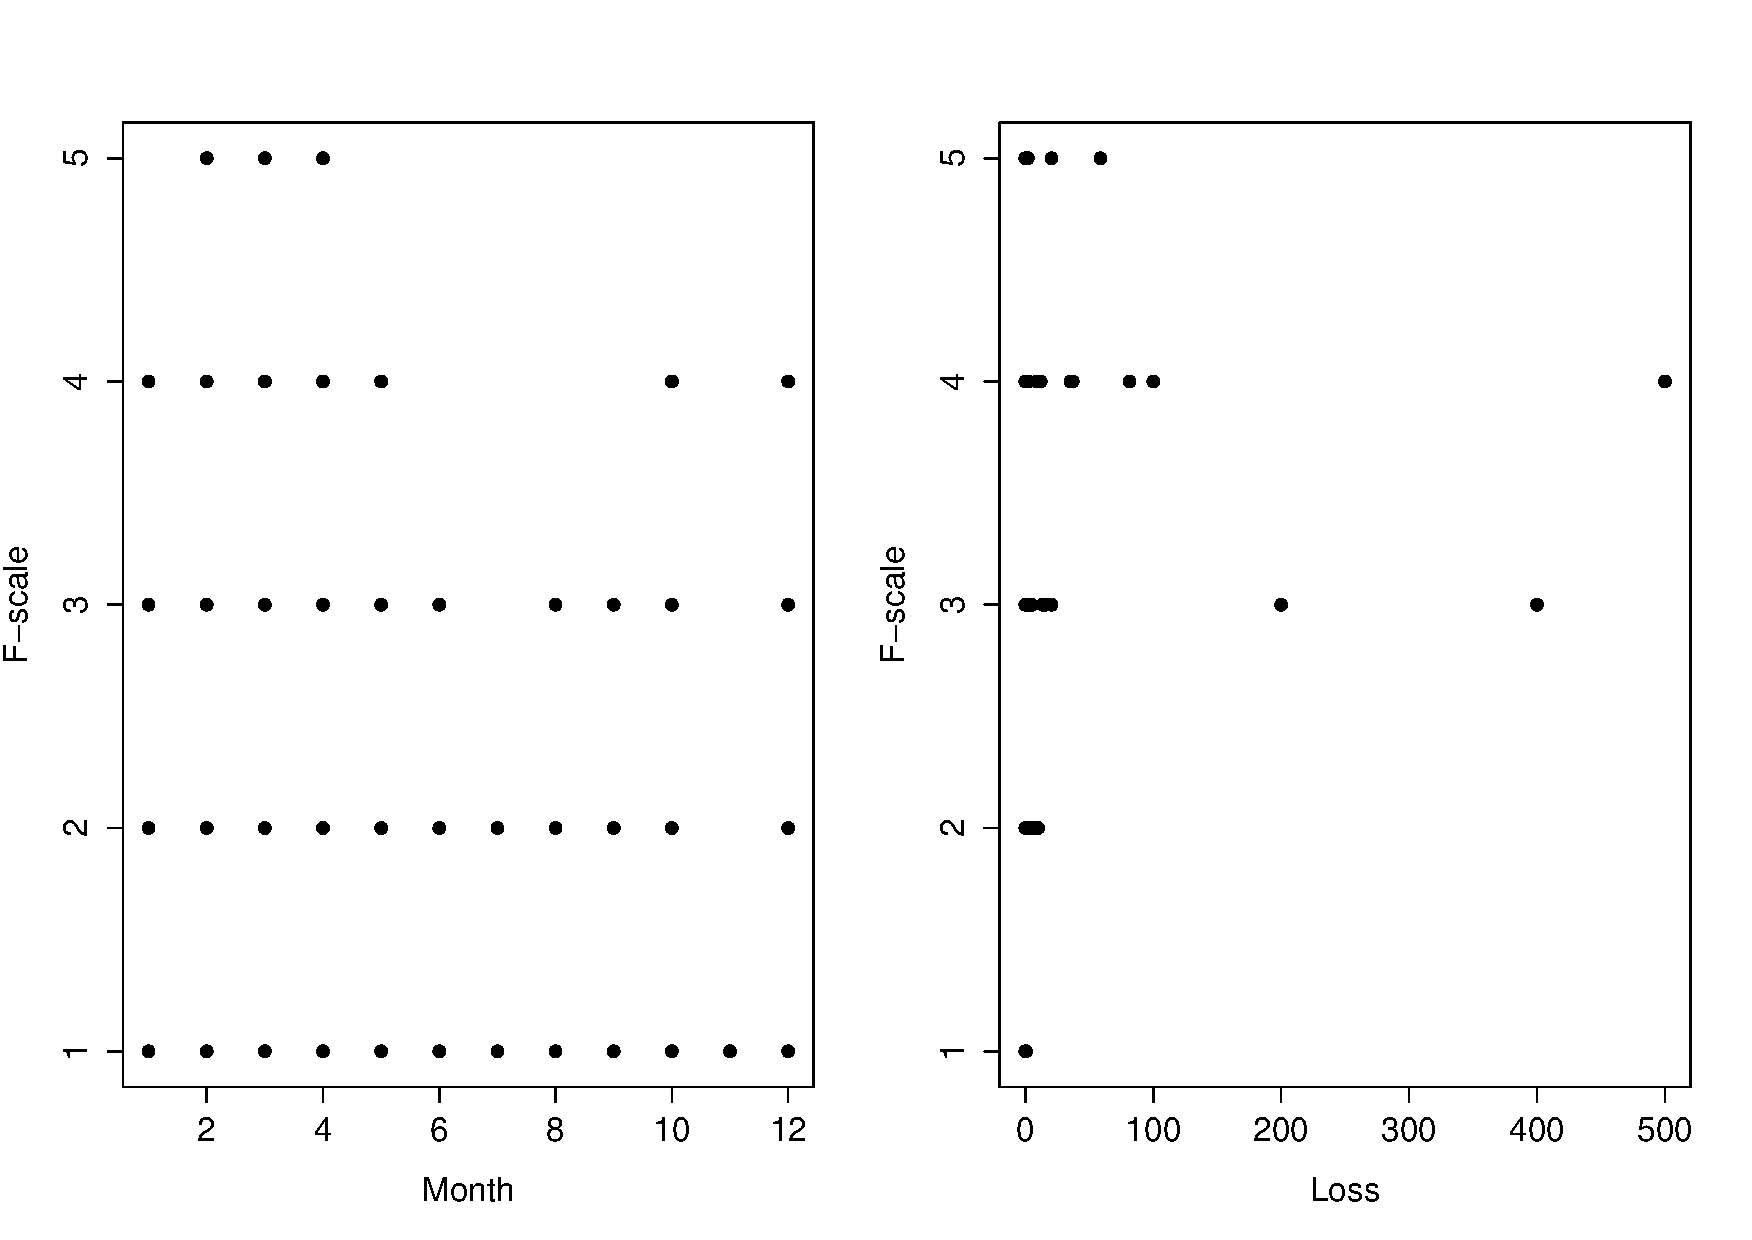
\includegraphics[scale=.4]{raw/dat.pdf}
        \end{figure}
      }

     \frame{
        \frametitle{Germination Rates}
        \begin{figure}
          \includegraphics[scale=.4]{raw/pairs.pdf}
        \end{figure}
     }
  
    \section{Model: Logistic Regression Model} 
      \frame{
        % Birds Eye:
        \frametitle{Logistic Regression Model (Linear)}
        \begin{align*}
          Y_i & \overset{ind}{\sim} \text{Bernoulli}(p_i) \\
          log\left(\frac{p_i}{1-p_i}\right) & = \bm{x_i^\prime\beta} \\
          \imp p_i & = \frac{e^{\bm{x_i^\prime\beta}}}{1+e^{\bm{x_i^\prime\beta}}}
        \end{align*}
        \wl
        where $p_i = P(Y_i=1)$
      }

      \frame{
        % Data independent (experiment)
        % But Data not linear: From plot of data. So: 
        \frametitle{Logistic Regression Model (Nonlinear)}
        \begin{align*}
          Y_i & \overset{ind}{\sim} \text{Bernoulli}(p_i) \\
          log\left(\frac{p_i}{1-p_i}\right) & = (ns(\bm ns(x_i)))^\prime\beta \\
          \imp p_i & = \frac{e^{\bm{ns(x_i)^\prime\beta}}}{1+e^{\bm{ns(x_i)^\prime\beta}}}
        \end{align*}
        \wl
        where $p_i = P(Y_i=1)$
      }

      \frame{
        \frametitle{Model}
        \begin{itemize}
        \item[+] Model is flexible
        \item[-] Number of knots needs to be predetermined
        \end{itemize}
      }


  \section{Results}
    \frame{
      \frametitle{Model}
      \begin{center}
        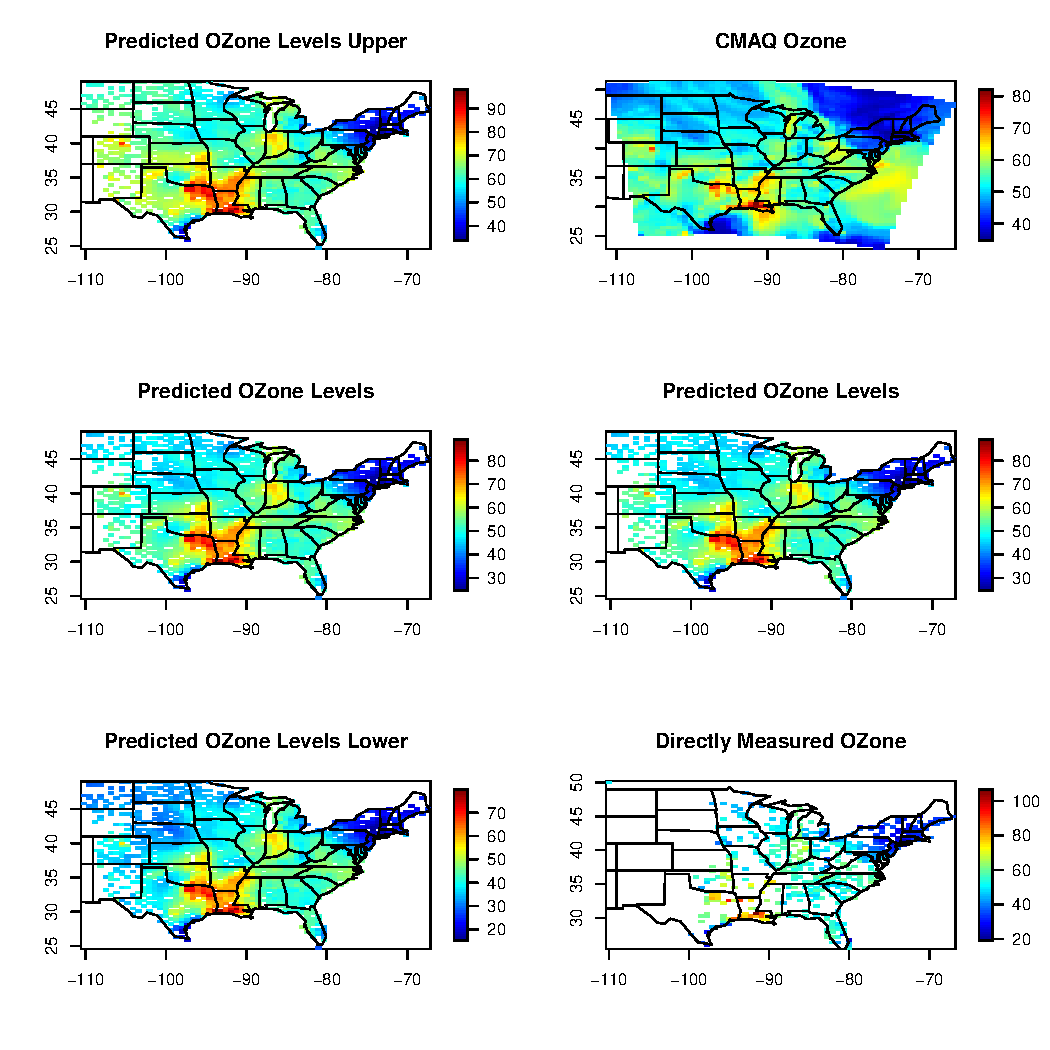
\includegraphics[scale=.37]{raw/all.pdf} 
      \end{center}  
      \input{raw/err.tex}
    }

    \frame{
      \frametitle{Effect of Chilling Time}
      Models to compare for every pair of populations: \\
        \begin{align*}
          log\left(\frac{p_i}{1-p_i}\right) & = \beta_0 + pop_i\beta_1 + 
                                                ns(chill_i)\beta_2 + 
                                                pop_i ns(chill_i)\beta_3 \\
          log\left(\frac{p_i}{1-p_i}\right) & = \beta_0 + ns(chill_i)\beta_2
        \end{align*}

    }

    \frame{
      \frametitle{Effect of Chilling Time}
      \begin{center}
        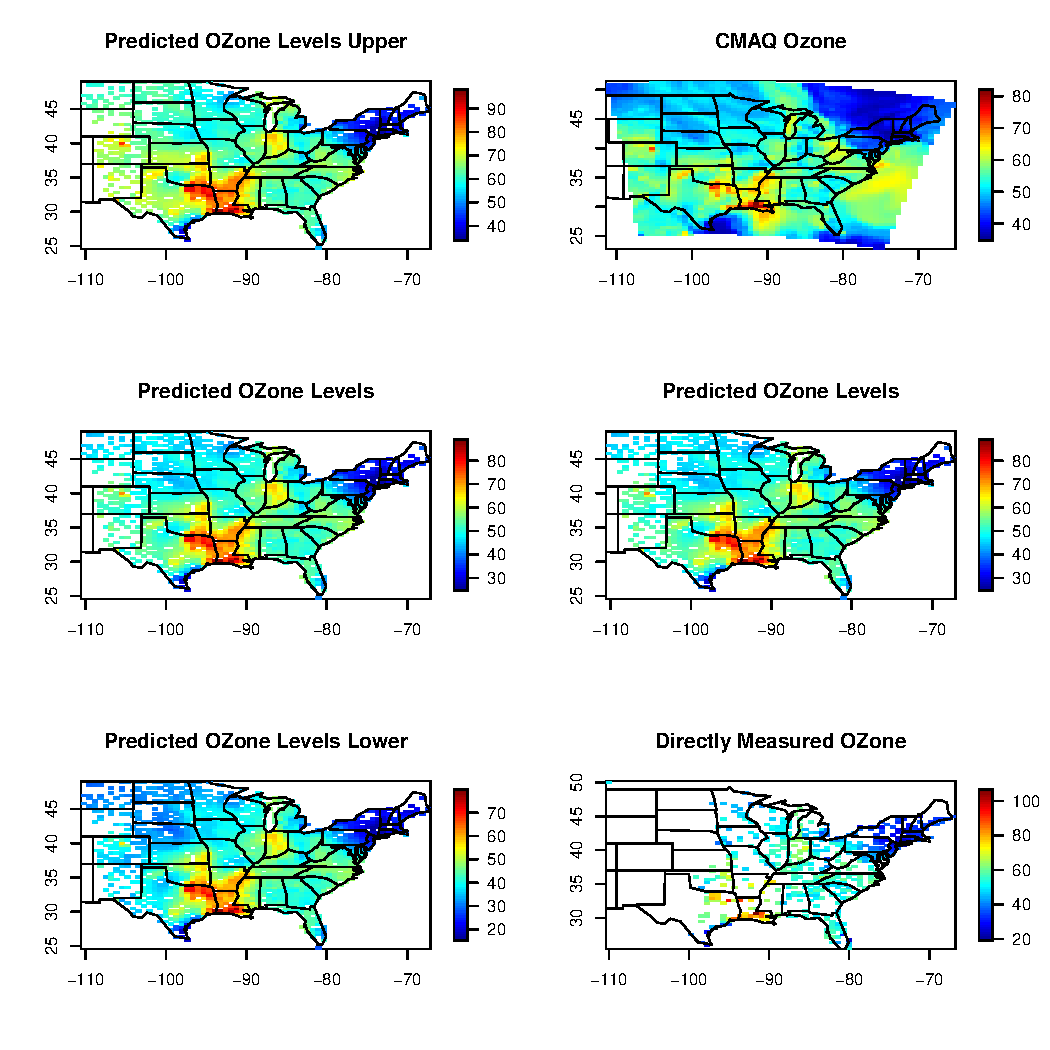
\includegraphics[scale=.37]{raw/all.pdf} 
      \end{center}  
      \tiny
      Populations that respond similarly to chilling time: 
      (3,2), (4,2), (10,4), (7,6), (10,6), (11,6), (10,7), (11,7), (11,10)
    }

    \frame{
      %I got these by bootstrapping:
      %  - sample data with replacement
      %  - fit model
      %  - find the mode of the predictions
      %  - the mean is the estimate
      %  - the standard deviation is the se
      \frametitle{Ideal Chilling Time}
      \input{raw/best.chill.tex}
    }

    \frame{
      \frametitle{Ideal Chilling Time}
      \begin{figure}
        \centering
        \includegraphics[scale=.4]{raw/bct.pdf}
      \end{figure}
    }

    \frame{
      \frametitle{Effect of Decrease in Chilling Time from 10 to 8 Weeks}
      \input{raw/effect.10.to.8.tex}
    }
    \frame {
      \frametitle{Effect of Decrease in Chilling Time from 10 to 8 Weeks}
      \begin{figure}
        \centering
        \includegraphics[scale=.4]{raw/eff.pdf}
      \end{figure}

    }
  \section{Conclusions}
    \frame{
      \frametitle{Conclusions}
        \begin{itemize}
          \item Populations: (3,2), (4,2), (10,4), (7,6), (10,6), 
                             (11,6), (10,7), (11,7), (11,10) are the same.
          \item Ideal Chilling Time: 11.5 (9.908898, 13.097589)
          \item Effect of Chilling Time Decrease on Germination Rates: 
                -0.041 (-0.066 -0.017)
        \end{itemize}
    }

  \section{Future}
    \frame{
      \frametitle{Future}
        \begin{itemize}
          \item Try Smoothing Splines
        \end{itemize}  
    }
  
    \frame {
      \frametitle{The End}
      \begin{center}
        \large{Thanks for the great semester!}
      \end{center}   
    }

\end{document}
